\section{User Interface}

\subsection{Main Page}

\begin{figure}[H]
    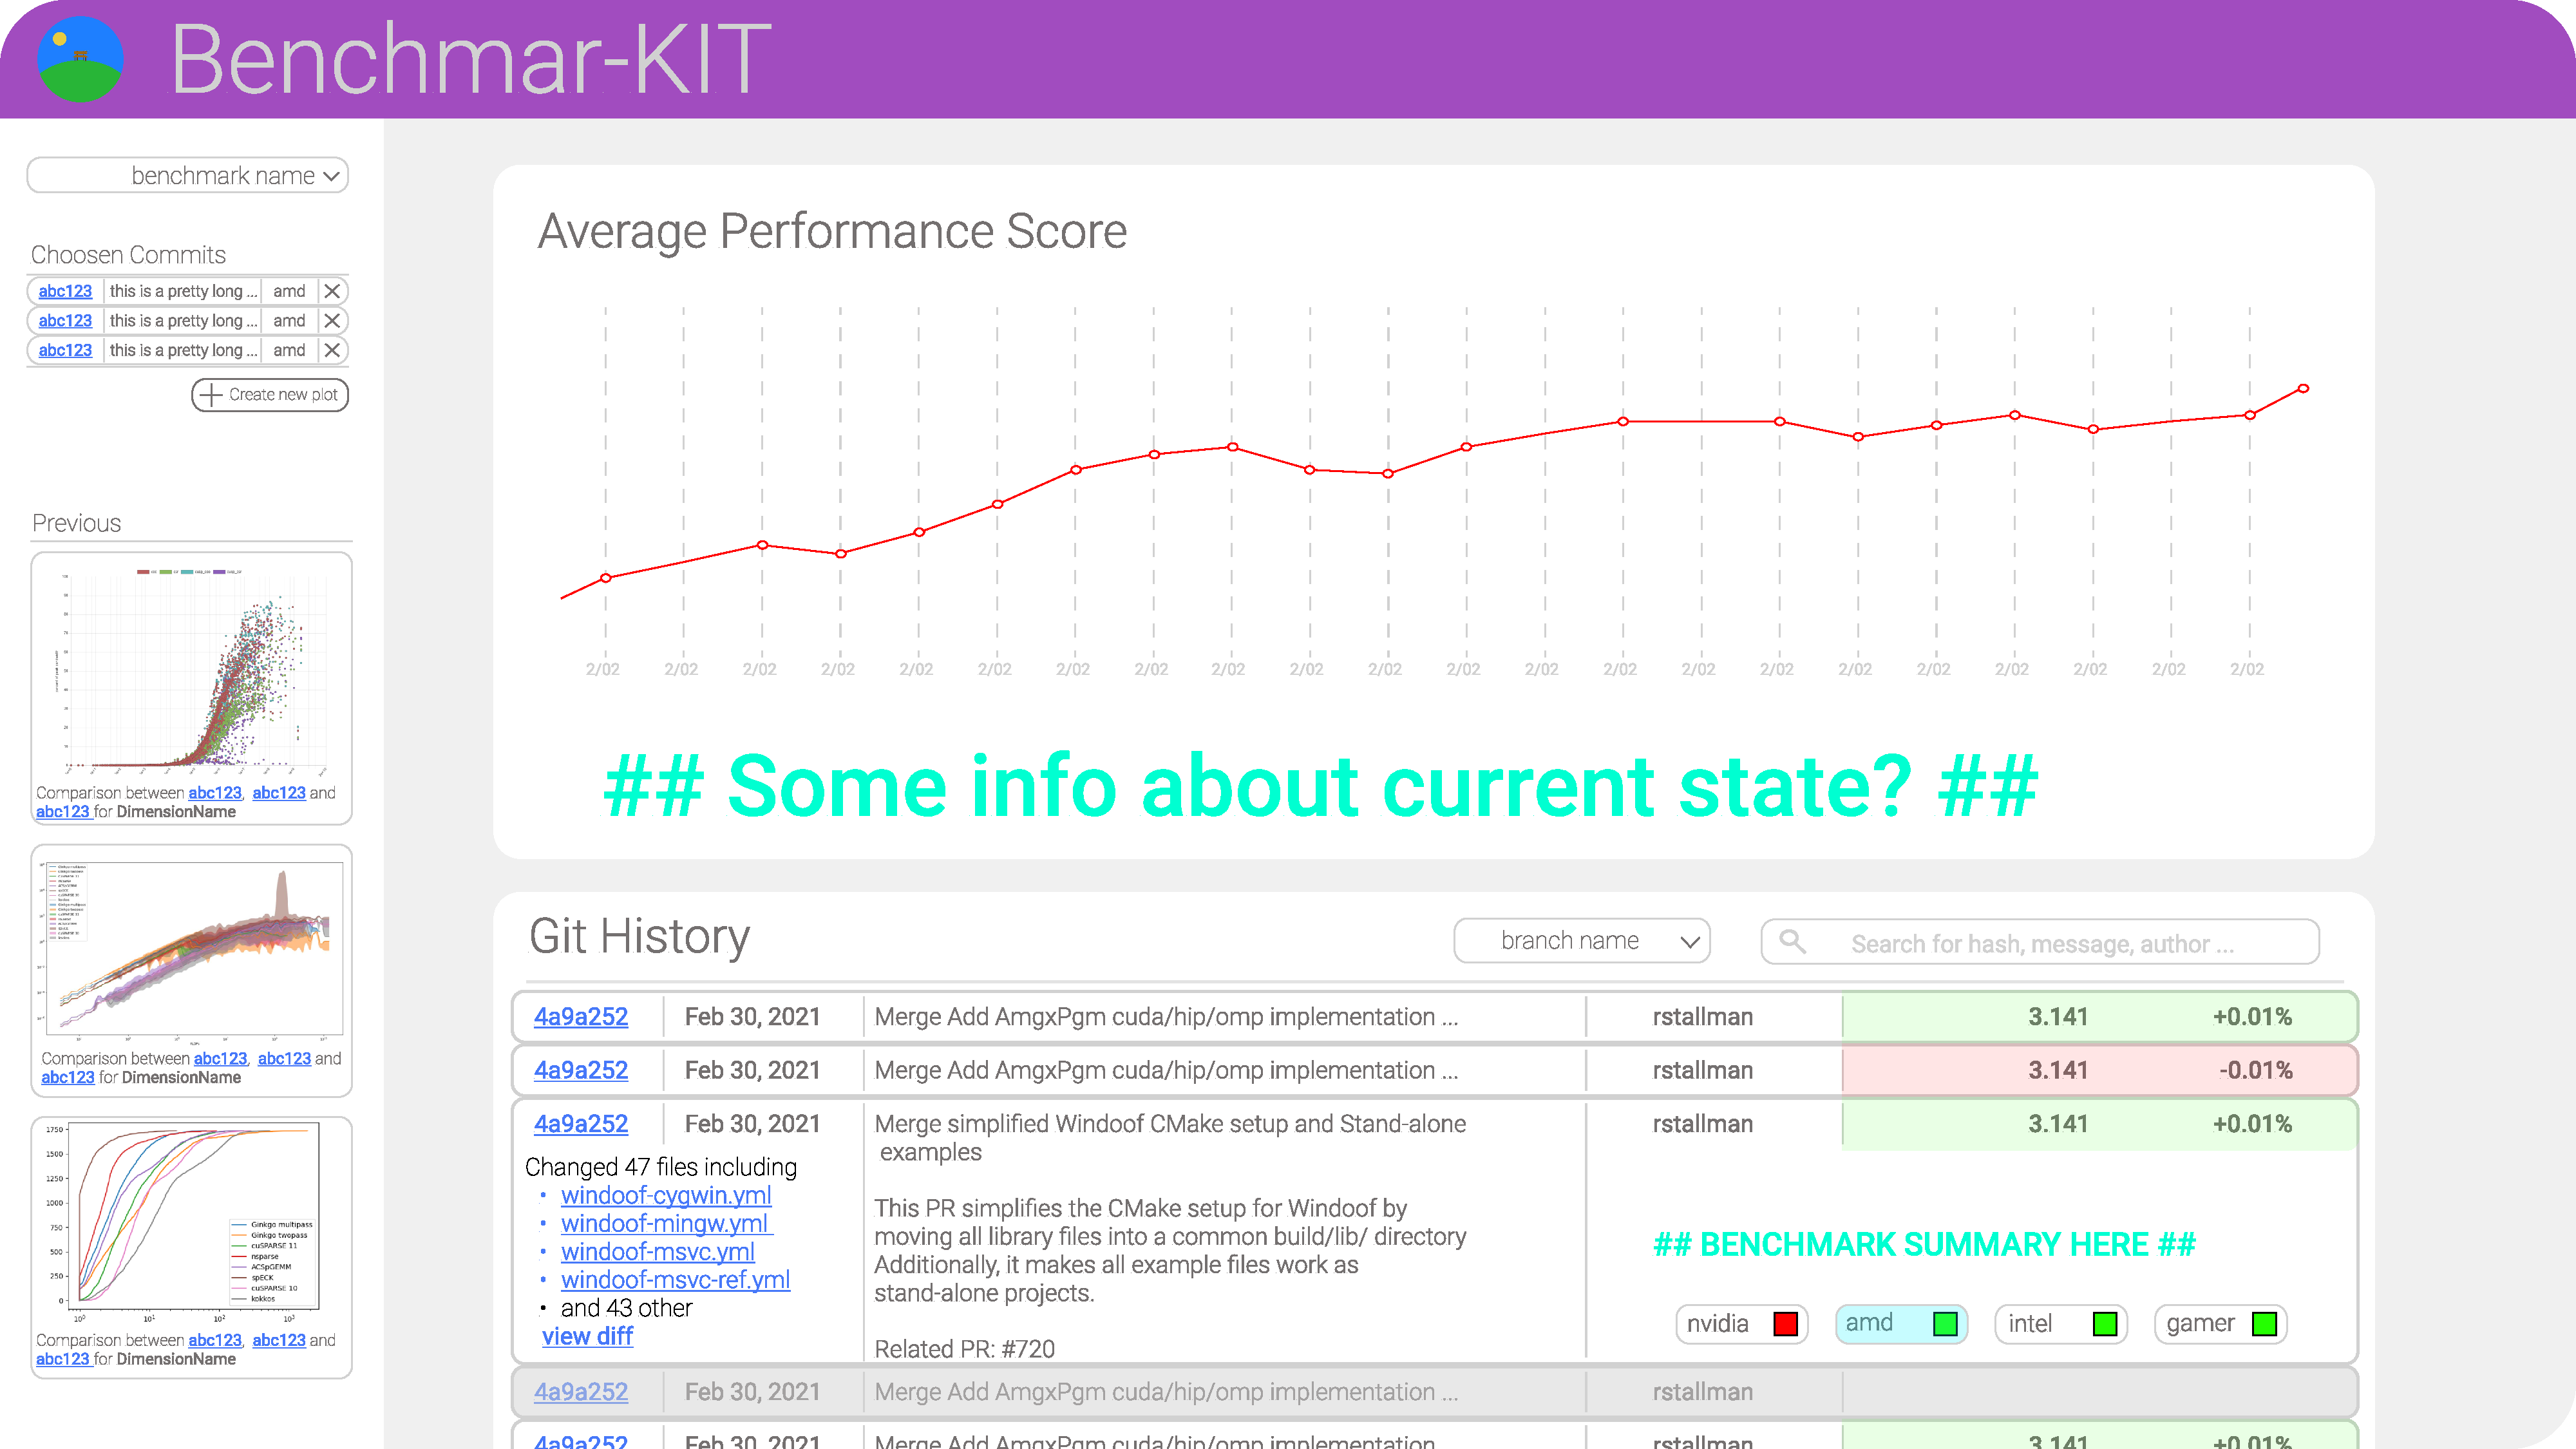
\includegraphics[width=\textwidth]{MainPage.pdf}
    \caption{Main page}
    \label{ui:main}
\end{figure}

The main page consists of an overview of the change history. The change history gets represented by list of changes. Every entry contains information about the changes such as hash, date and commit message. The user adds changes by selecting a specific change and then choosing a specific device. Selected changes get added to the list on the left. Benchmark type and branch can be chosen via dropdown menus. The user can open the configuration popup by selecting the \enquote{Create New Plot} option.

\subsection{Configuration Popup}

\begin{figure}[H]
    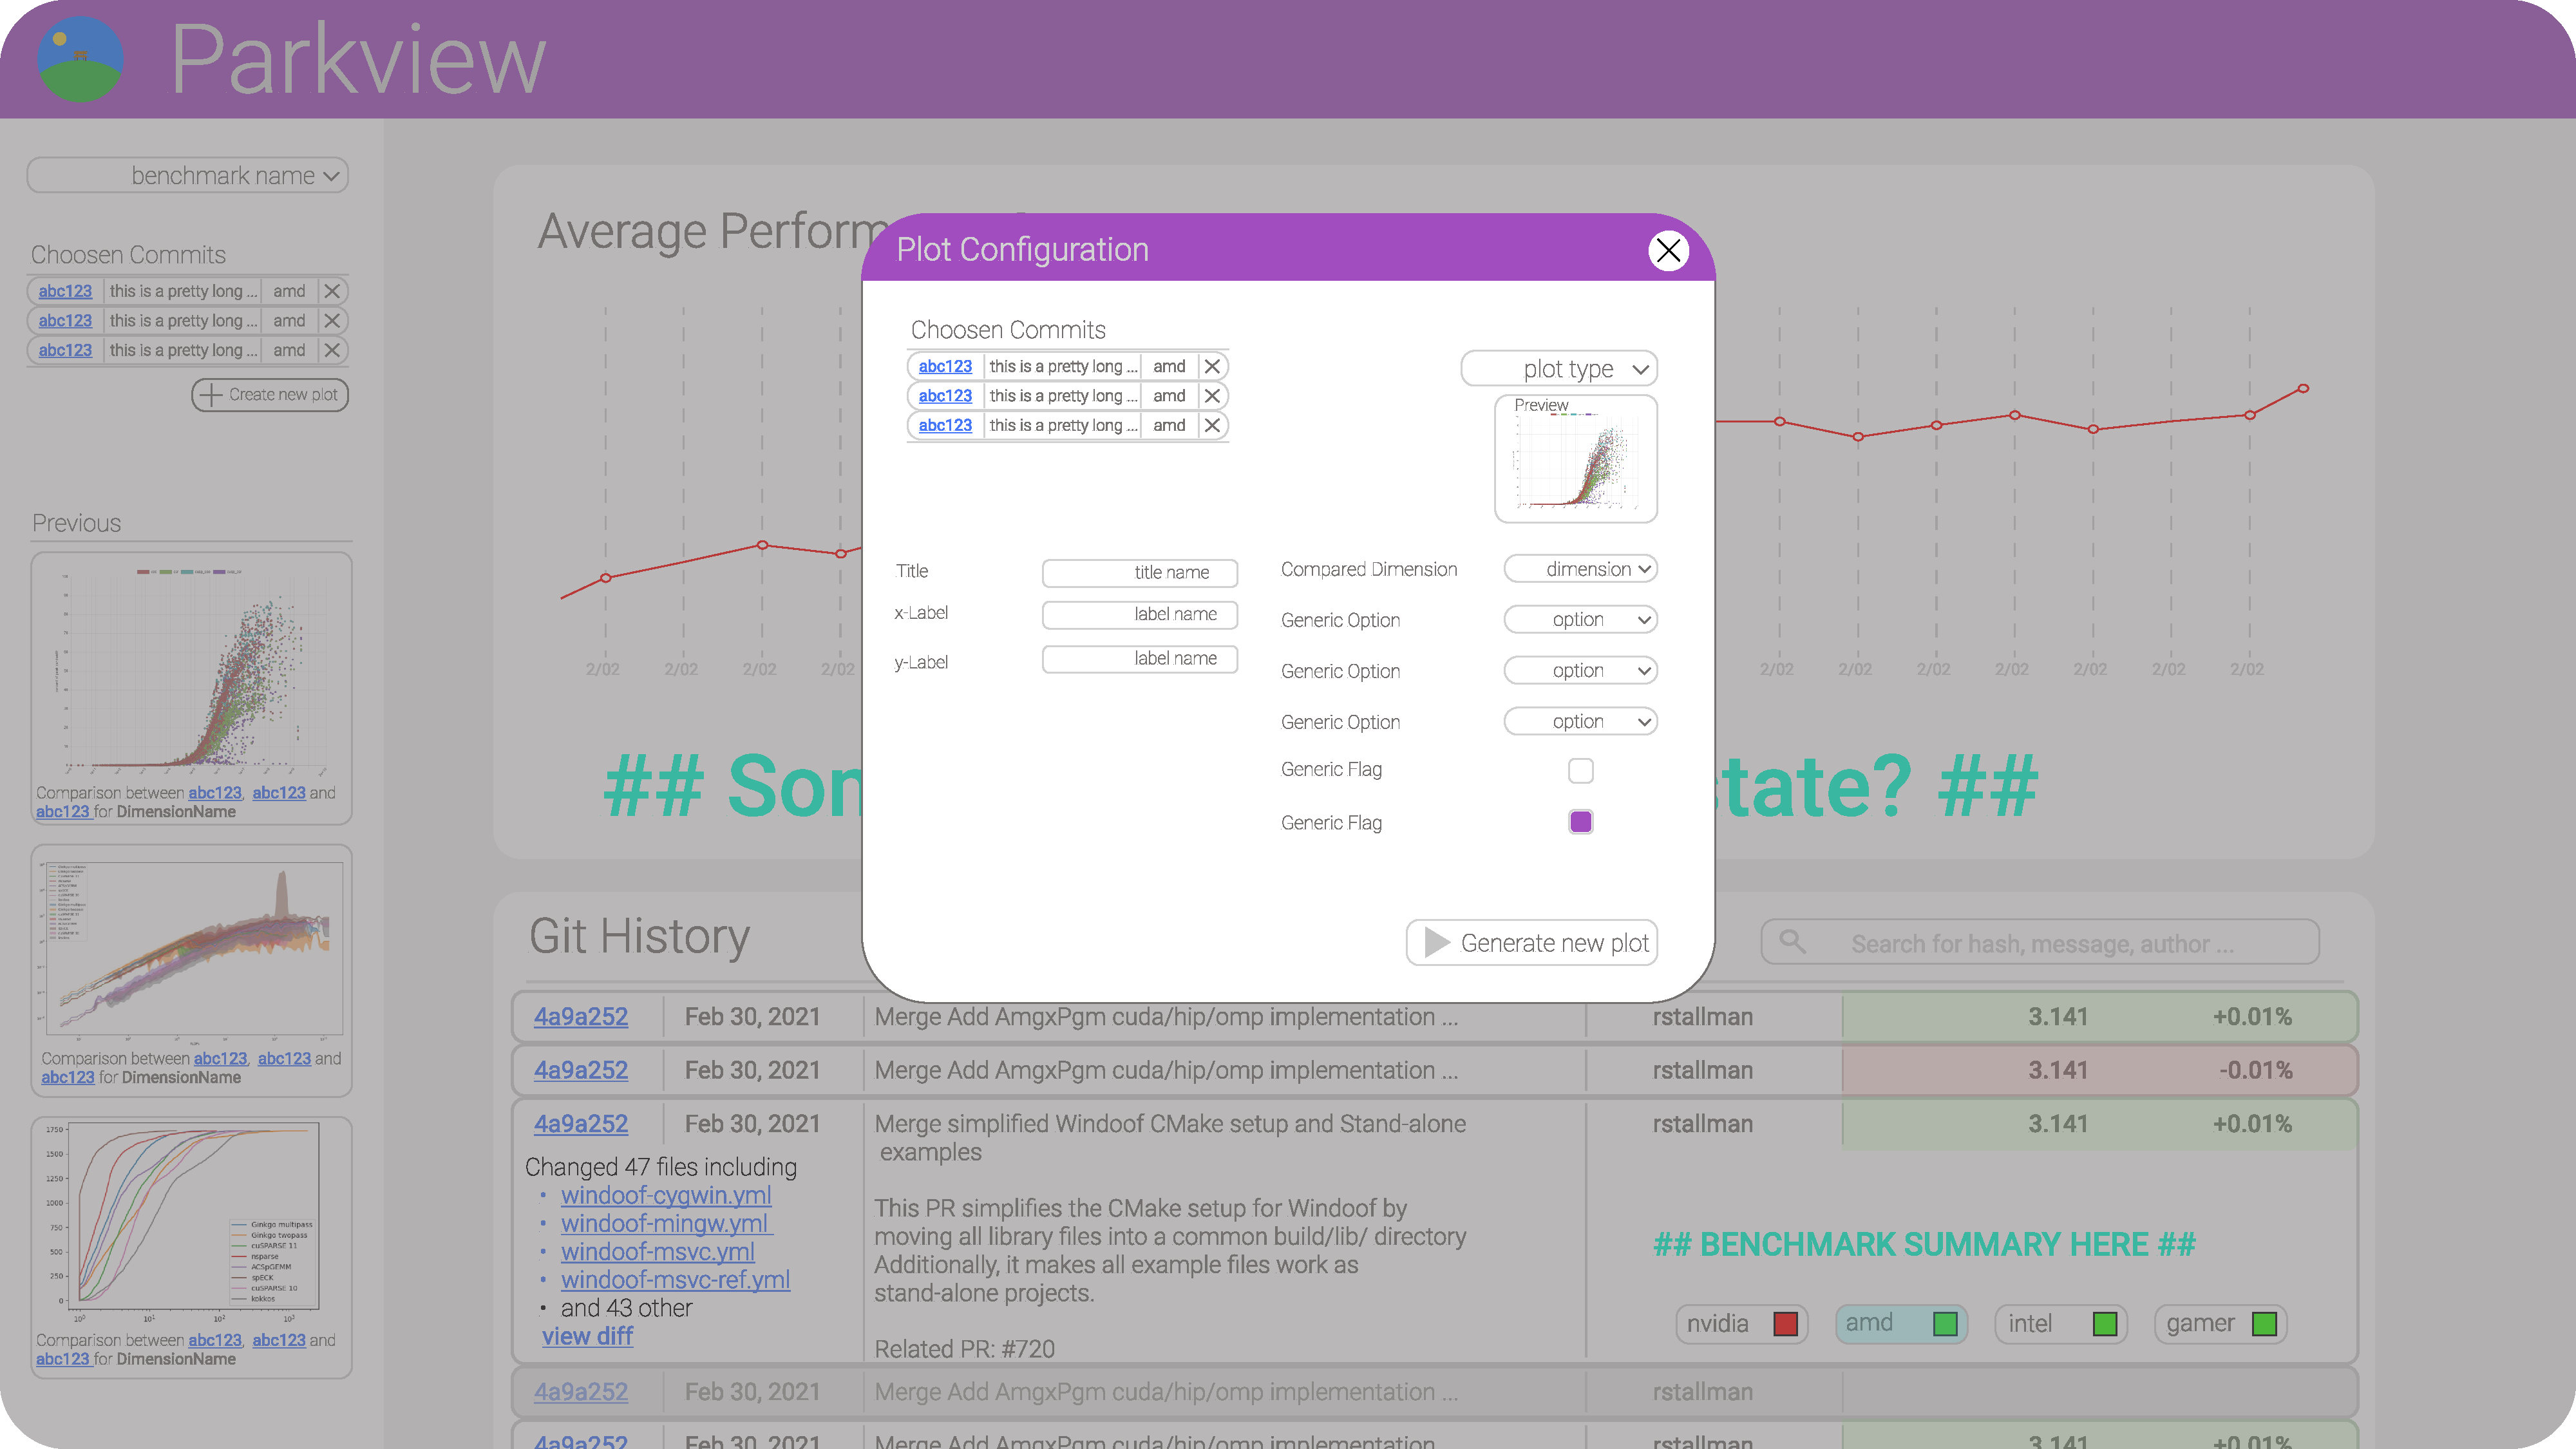
\includegraphics[width=\textwidth]{ConfigurationPopup.pdf}
    \caption{Configuration Popup}
    \label{ui:config}
\end{figure}

The configuration Popup contains all options for configuring the \gls{visualization}. Categorical options can be chosen via dropdown menus, flags can be set with checkboxes and any other options can be set using textboxes. The popup can be closed using the cross in the top right. A small preview of the plot type gets displayed under the option for plot types. By selecting the \enquote{Generate New Plot} option the user starts the generation of the \gls{visualization} and webapp displays it to the user.

\subsection{Plot View}

\begin{figure}[H]
    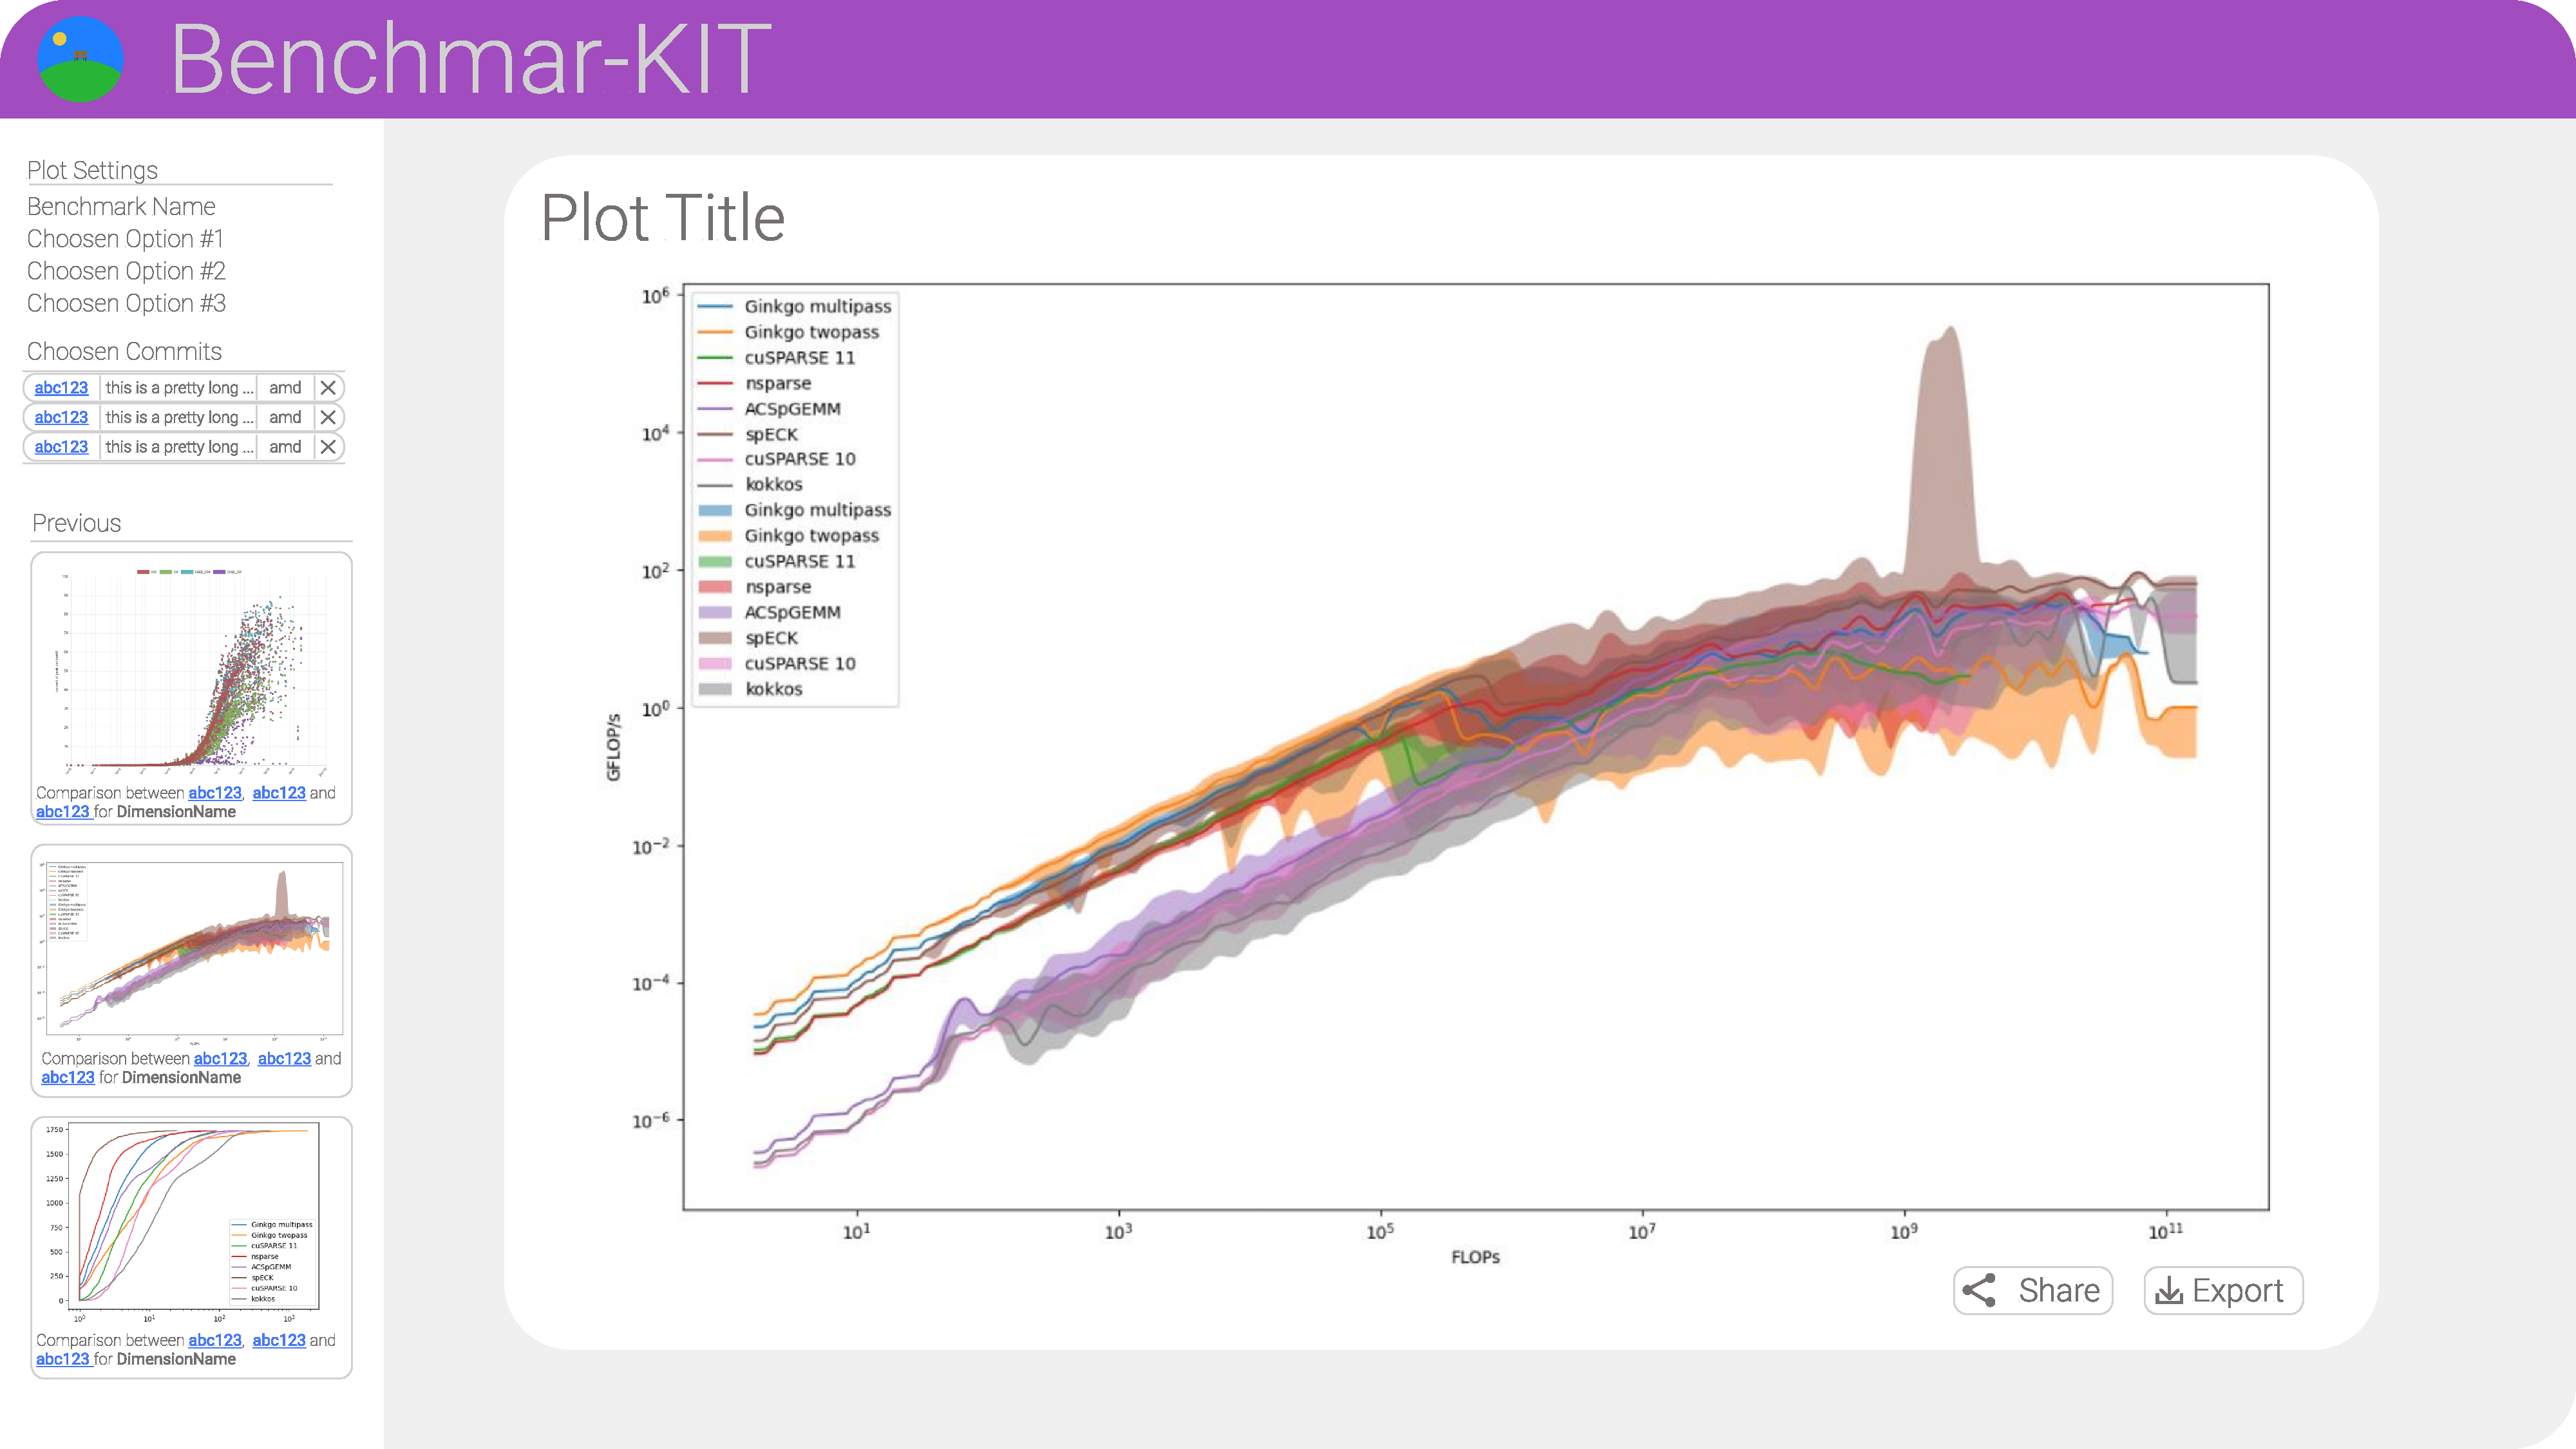
\includegraphics[width=\textwidth]{PlotView.pdf}
    \caption{View of a \gls{visualization}}
    \label{ui:plot}
\end{figure}

The plot view allows the user to inspect the \gls{visualization}. The user can share the \gls{visualization} by selecting the \enquote{Share} option. He can also download it by selecting the \enquote{Export} option. Selecting the logo on the top left redirects the user to the main page.
